\documentclass[11pt,a4paper]{article}
\usepackage[margin=1in]{geometry}

\usepackage{pgfplots}
\pgfplotsset{width=4in,compat=1.9}

\usepackage{float}

\begin{document}


\begin{titlepage}

% You need to edit the details here

\begin{center}
{\LARGE University of Sheffield}\\[1.5cm]
\linespread{1.2}\huge {\bfseries Assignment 1: Document Retrieval}\\[1.5cm]
\linespread{1}
\includegraphics[width=5cm]{images/tuoslogo.png}\\[1cm]
{\large COM3110 Text Processing (AUTUMN 2020-21)}\\[1cm]
{\Large Boxuan Shan}\\[6cm]
\large Department of Computer Science\\[1cm]
\today
\end{center}

\end{titlepage}

% -------------------------------------------------------------------
% Declaration
% -------------------------------------------------------------------

\newpage
\section*{\Large Implementation}

In this assignment, I implemented a Retrieve class for the IR that can retrieve documents by a query with three different weighting schemes: binary, tf, and tfidf. In this class, there are three private methods: forQueryBinary, forQueryTf, forQueryTfidf, which correspond to the three different weighting schemes. These three methods take a query as a parameter and return a list of retrieved docid. 

The private method forQueryBinary calls the private method rankByCosSim, which takes a query and a weighting callback as parameters. First, rankByCosSim calls the private method findRelated to find all related documents that contain the terms in the query, and then calculates the cosine distance between the document vector $\vec{d}$ and the query vector $\vec{q}$ for each related document as the similarity of the document and the query, where the value of each term in the vectors $\vec{d}$ and $\vec{q}$ will be evaluated by the weighting callback. In this case, the weight callback will be binaryWeighting, which will return a integer 1 for every term that exist in the context. Finally, the documents are sorted according to similarity and returned as the result. The mathematical expression of cosine distance is as follow:

\begin{equation}
    sim(\vec{q},\vec{d})=cos(\vec{q},\vec{d})=\frac{\sum_{i=1}^{n}q_id_i}{\sqrt{\sum_{i=1}^{n}q_i^2}\sqrt{\sum_{i=1}^{n}d_i^2}}
\end{equation}

where $\vec{q}$ is the vector of the query, $\vec{d}$ is the vector of the document. Since $\vec{q}$ is constant for one query, the calculation of similarity can be simplified to the following if the query is the same:

\begin{equation}
    sim(\vec{q},\vec{d})=\frac{\sum_{i=1}^{n}q_id_i}{\sqrt{\sum_{i=1}^{n}d_i^2}}
\end{equation}

The private method forQueryTf will also call the private method rankByCosSim, but will use tfWeighting as the weighting callback. This callback will return the number of times the term appears in the context (a.k.a. TF or Term Frequency) as the weighting result.

The private method forQueryTfidf will call the private method rankByCosSim as well, but the weighting callback will be tfidfWeighting in this case. This callback will count and store the number of documents in this document collection, and then weighting the terms by frequency in context vs in collection (a.k.a. TF.IDF) as the return. The mathematical expression of TF.IDF is as follows:

\begin{equation}
    tf.idf_{w,d,D} = freq_{w,d}\cdot log\frac{|D|}{df_{w}}
\end{equation}

where $freq_{w,d}$ is the number of times term $w$ occurs in document $d$, $|D|$ is the total number of documents in the collection $D$, $df_{w}$ is the number of documents in the document collection $D$ containing the term $w$.

\section*{\Large Evaluation}

The IR system is used to process a set of queries on the CACM document collection under a range of configurations, and then the results are evaluated by F-measure. Weighting schemes include Binary, TF and TF.IDF. Preprocessing methods include Raw, Stemming only, Stoplist only, and Both. The evaluation result is shown in the Table \ref{tab:result}.

\newpage

\begin{figure}[H]
    \centering
    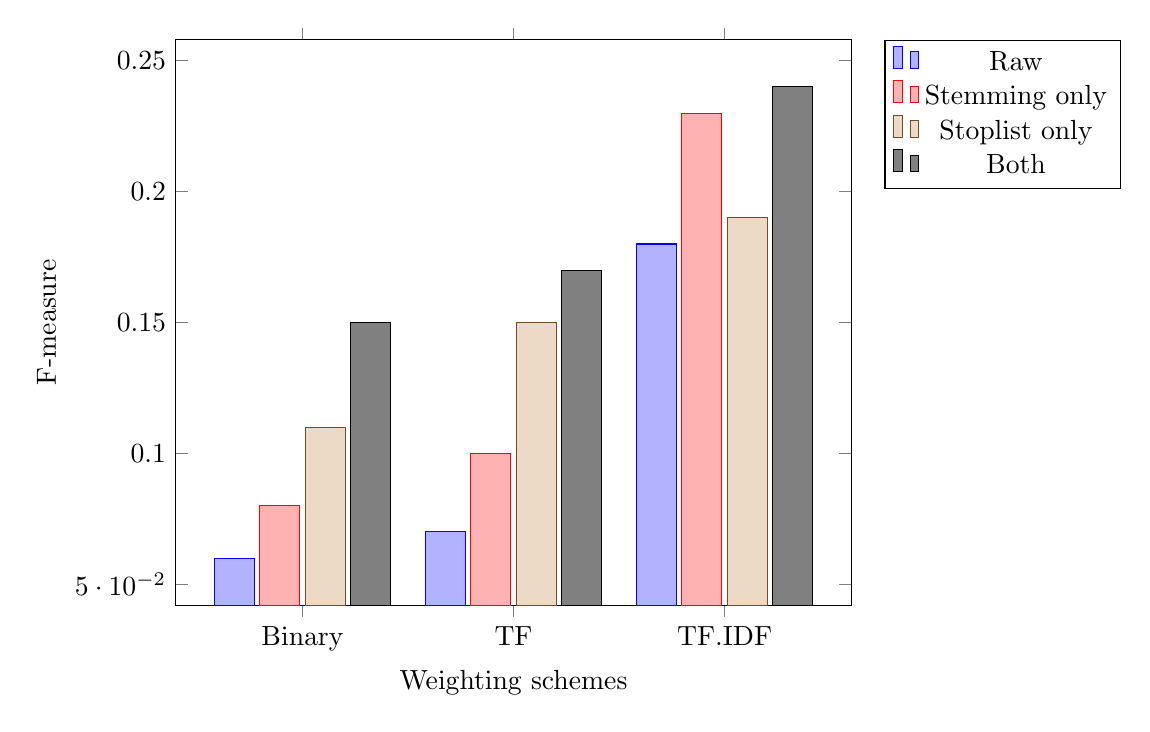
\begin{tikzpicture}
        \begin{axis}
        [
            symbolic x coords={Binary,TF,TF.IDF},
            xtick=data,
            ylabel=F-measure,
            xlabel=Weighting schemes,
            legend style={at={(1.4,1)}},
            ybar,
            bar width=0.2in,
            enlarge x limits=0.3
        ]
        \addplot coordinates{ (Binary,0.06) (TF,0.07) (TF.IDF,0.18) };
        \addplot coordinates{ (Binary,0.08) (TF,0.10) (TF.IDF,0.23) };
        \addplot coordinates{ (Binary,0.11) (TF,0.15) (TF.IDF,0.19) };
        \addplot coordinates{ (Binary,0.15) (TF,0.17) (TF.IDF,0.24) };
        \legend{Raw, Stemming only, Stoplist only, Both}
        \end{axis}
    \end{tikzpicture}
    \caption{F-measures of IR system under a range of configurations.}
    \label{fig:result}
\end{figure}


\begin{table}[H]
    \centering
    \begin{tabular}{|l|l|l|l|}
        \hline
        &Binary&TF&TF.IDF\\
        \hline
        Raw&0.06&0.07&0.18\\
        \hline
        Stemming only&0.08&0.10&0.23\\
        \hline
        Stoplist only&0.11&0.15&0.19\\
        \hline
        Both&0.15&0.17&0.24\\
        \hline
    \end{tabular}
    \caption{F-measures of IR system under a range of configurations.}
    \label{tab:result}
\end{table}

\section*{\Large Analysis}

From Figure \ref{fig:result}, in general, in terms of the weighting scheme, TF.IDF has the best accuracy, followed by TF, and the worst is Binary. At the same time, the method of preprocessing will also affect the accuracy of retrieval. Usually, when both stremming and stoplist are used, the accuracy is the highest, followed by the case where only stoplist is used, and then the case where only stemming is used. The accuracy is the worst when using raw data.

However, when TF.IDF is used as the weighting scheme, the accuracy of stemming only case is better than the accuracy of stoplist only case. This means that with the absence of the stoplist, TF.IDF can still achieve considerable accuracy. This should be because this weighting scheme reduces the weight of terms that frequently appear in the document collection, which is to some extent the same as the purpose of stoplist, thereby reducing the detrimental impact on the accuracy when stoplist is absent.

In summary, using TF.IDF weighting scheme combined with both Stoplist and Stemming preprocessing can usually get the best retrieval results.

\end{document}
